\subsection{CONFIGURACIÓN ARCHIVO INICIAL}
El proyecto contendrá un nodo raíz el cual será el que tendrá los llamados al conjunto de elementos que tendrá nuestra librería. Anteriormente se creó un directorio llamado “src” en la raíz de “crown”, dentro de “src” debemos crear un archivo llamado “index.js” este es un archivo de JAVASCRPT el cual definiremos como punto de inicio de webpack  y a partir de este buscará todas las importaciones de otros submódulos. Con el siguiente comando creamos el archivo requerido.
\newline
\newline
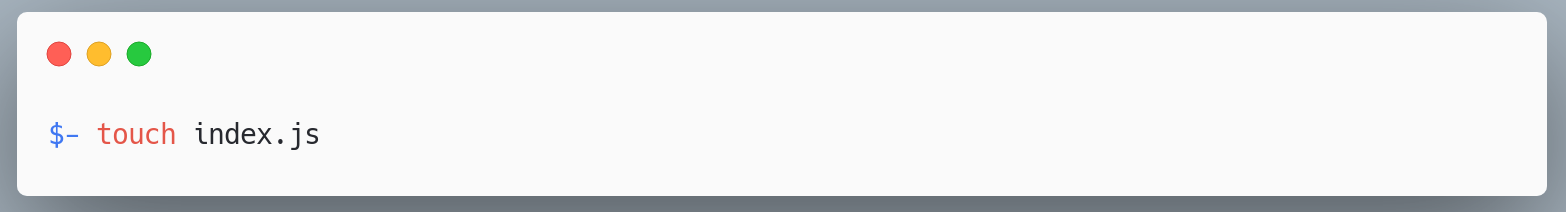
\includegraphics[width=1\textwidth]{./Imagenes/carbon.png}
\newline
\newline
Dentro de este archivo debemos poner el llamado a cada elemento que se vaya agregando a nuestra librería ( Botones, Campos de texto, Tablas etc.), en la siguiente ilustración se muestra la manera en que se deben agregar los elementos.
\newline
\newline
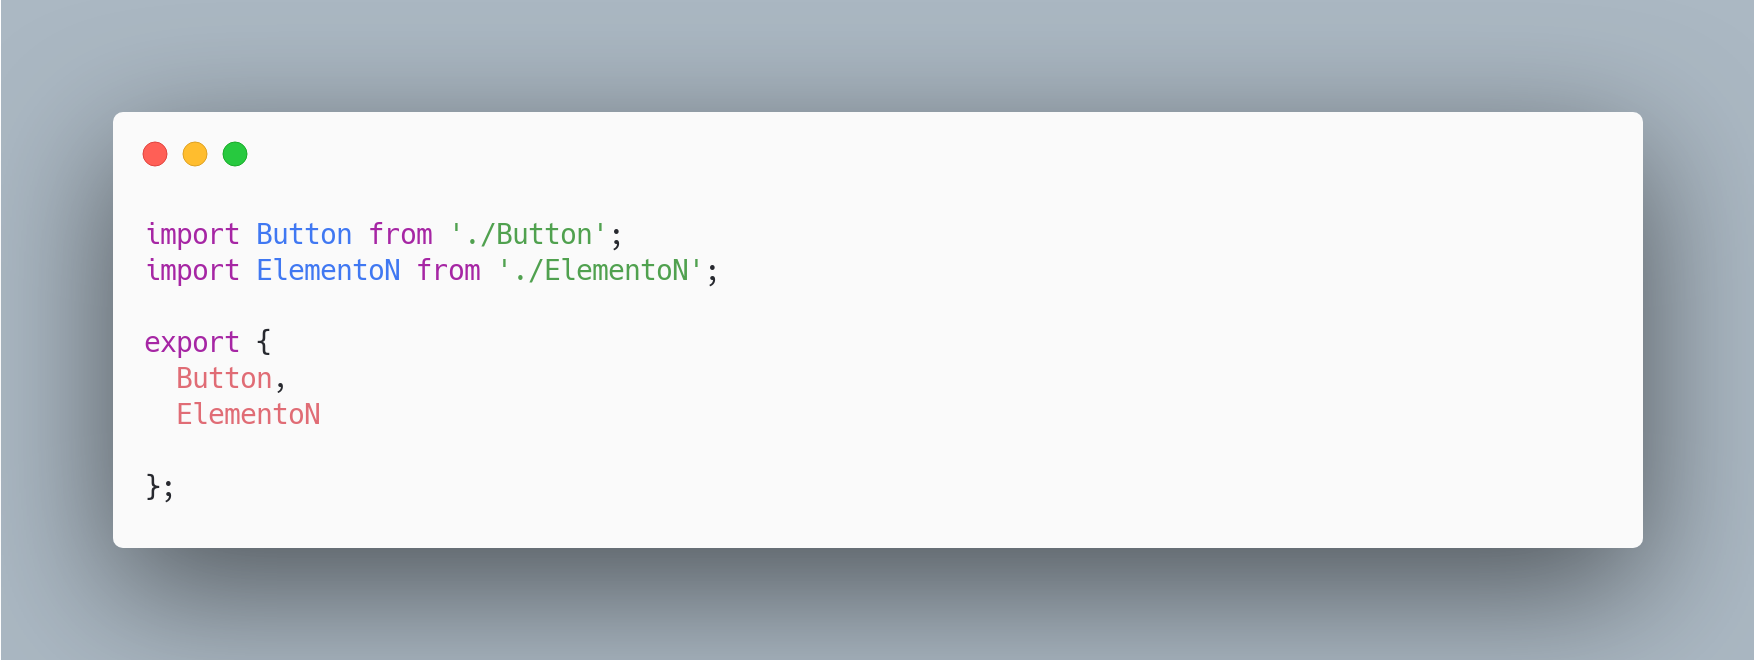
\includegraphics[width=1\textwidth]{./Imagenes/carbon-2.png}
\newline
\newline
El primer bloque de código muestra la importación de cada uno de los elementos a nuestro archivo index, y la segunda parte exportamos un objeto de JAVASCRIPT con cada uno de los elementos.
WEBPACK analiza cada elemento que se incluye en el objeto y busca el contenido existente dentro de cada uno.
Cada uno de los elementos que se necesita agregar deben estar situados a la misma altura del archivo “index.js” esto dentro del directorio “src” para que puedan ser procesados.



\subsection{ELEMENTO BOTÓN}
El primer elemento que vamos a agregar es el botón, para esto creamos un directorio llamado “Botton” de la siguiente manera.
\newline
\newline
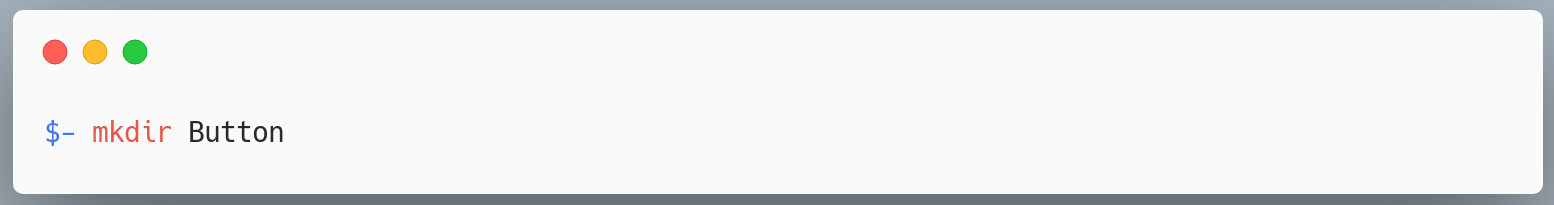
\includegraphics[width=1\textwidth]{./Imagenes/carbon-3.png}
\newline
\newline
Y dentro de este directorio crearemos dos archivo que son los que incluirán el núcleo de nuestro botón, el primer archivo se llamará “index.js ” esto es así ya que por defecto, cuando importas un archivo que está dentro de un directorio, JAVASCRIPT toma el que es llamado “index.js” y no es necesario especificar este dato, esto lo podemos ver de manera clara en el archivo inicial “index.js” que está al mismo nivel que el directorio “Botton”, el cual importa el elemento Botton pero no especifica el archivo. Este archivo solamente hace el llamado al segundo archivo “Botton.js” que es el que tiene el código fuente del botón. 
\newline
\newline
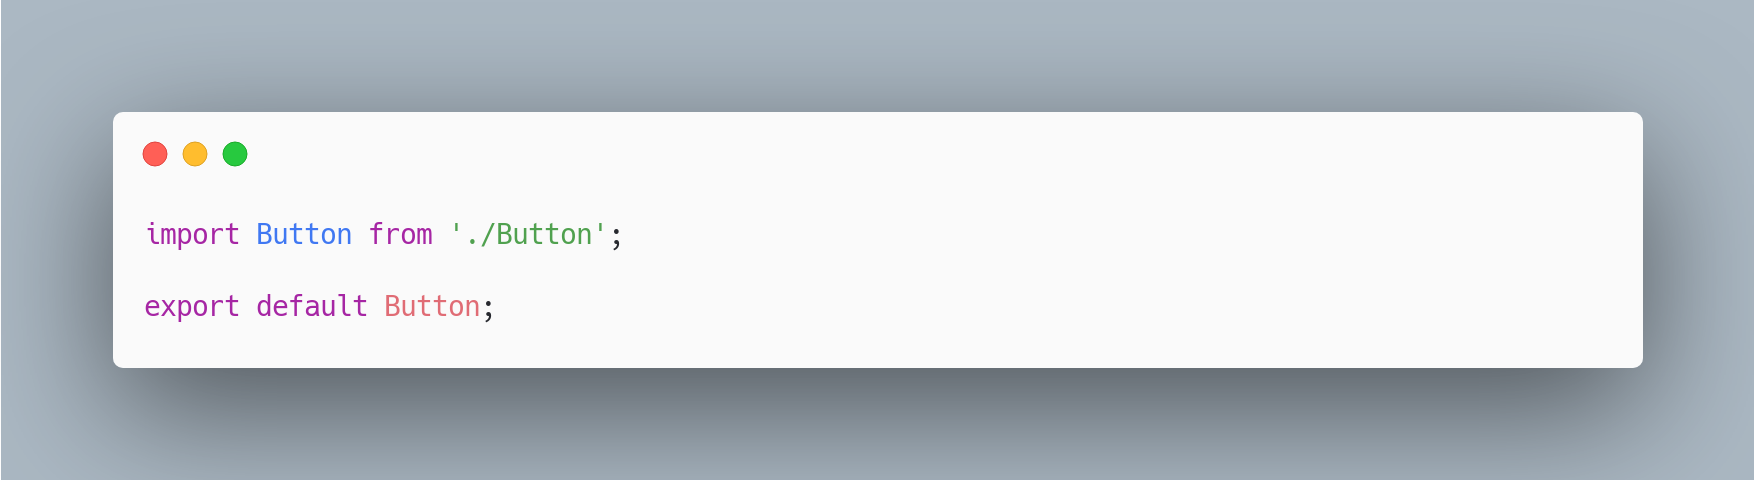
\includegraphics[width=1\textwidth]{./Imagenes/carbon-5.png}
\newline
\newline
El segundo archivo ya mencionado “Botton.js”  hace el render de nuestro botón, y gestiona la configuración que el usuario final quiera asignarle.
En la siguiente tabla se muestran los props ( configuración inicial  ) del botón.
\newline
\newline
\begin{center}
 \begin{tabular}{ | c |  p{5cm}  | c | p{3cm} |} 
 \hline
 \textbf{Nombre} &  \textbf{Uso} &  \textbf{ Tipo de dato} &  \textbf{Valor por defecto}\\ [0.5ex] 
 \hline\hline
text & Texto que mostrará el botón.  &  Cadena de texto. & Click me! \\  [2.5ex] 
 \hline
onClick & Es la función que ejecutará cuando se hace click. & Funcion. & Función vacía. \\[2.5ex] 
 \hline
color &  Es el color del botón. & Cadena de texto. & --blue-4 \\[3.5ex] 
 \hline
 textColor & Es el color del texto en el botón. &  Cadena de texto. & --white \\[2.5ex] 
 \hline
borderColor & Es el color del borde del botón. & Cadena de texto. & --blue-4 \\ [2.5ex] 
 \hline
 type & Es el tipo de botón. & Cadena de texto. & Default \\ [2.5ex] 
 \hline
 shape & Es la forma del botón. Estos valores agregaran una curvatura, tenemos Round y SemiRound uno mas curvo que otro. & Cadena de texto. & Round \\ [2.5ex] 
 \hline
 shadow & Especifica si el botón debe tener una sombra. & Cadena de texto. & Booleano. \\ [2.5ex] 
 \hline
\end{tabular}
\end{center}
\newline
\newline
\newline
Los tipos (type) de botones que podemos tener son los siguientes.
\begin{itemize}
\item \textbf{Default:} Es el botón que se recomienda usar como principal.
\item \textbf{Secondary:} Es recomendable usarlo si ya se usa un botón default, para cuidar la jerarquía visual.
\item \textbf{Text:} Este es un botón sin contorno, debe ser usado para acciones con poca importancia.
\end{itemize}
Los colores que se usan son una constante definida por la librería ya que se considera que son cromáticamente compatibles entre ellos, este tema se abordará más adelante.
A continuación se muestra un fragmento del código que permite agregar la configuración requerida.
\newline
\newline
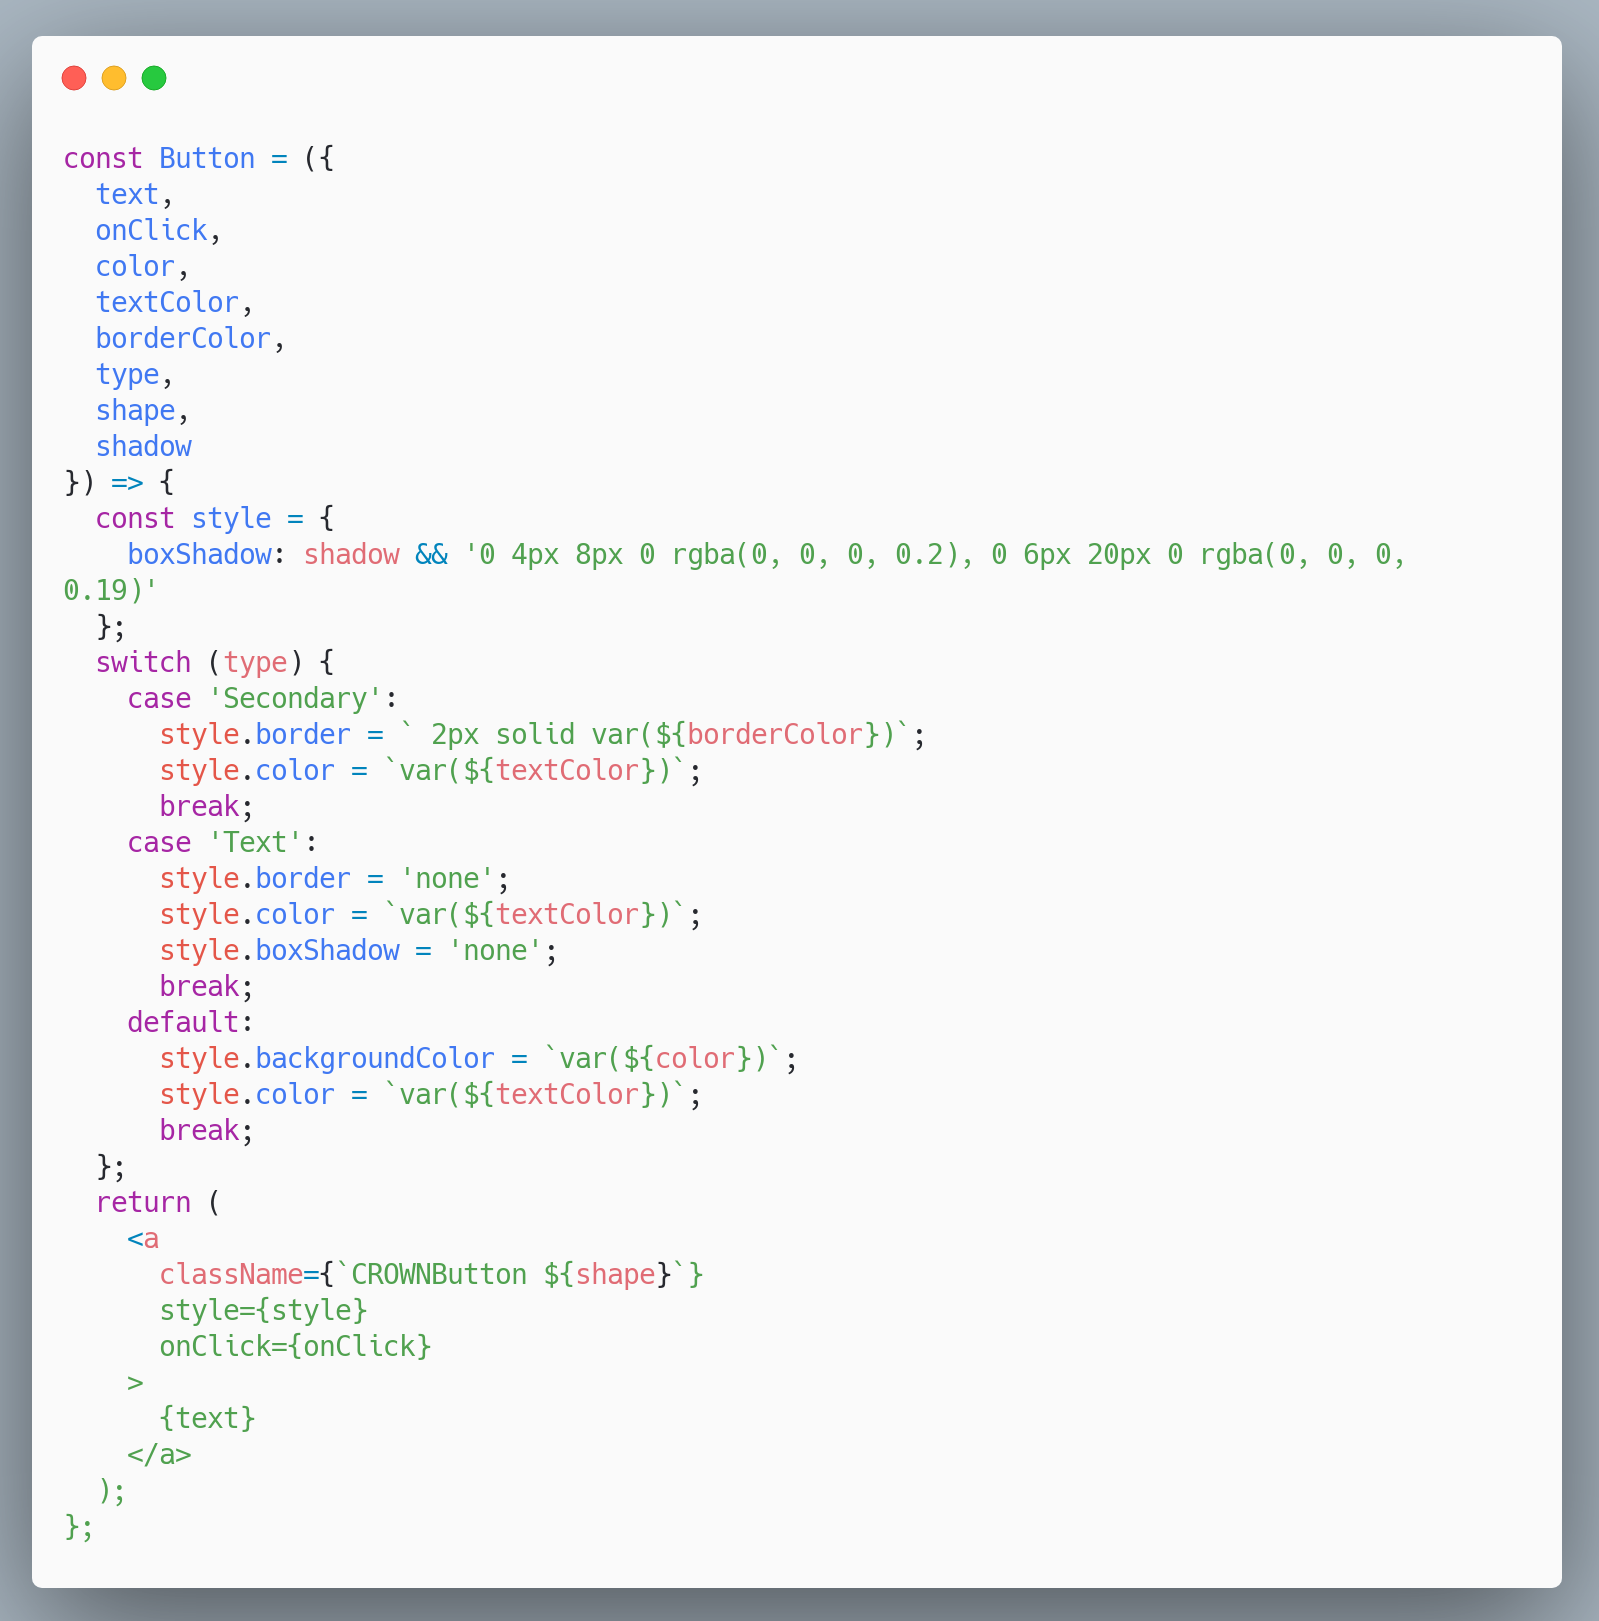
\includegraphics[width=1\textwidth]{./Imagenes/carbon-9.png}
\newline
\newline
En la primera parte podemos ver una lista de la configuración dada,  después definimos un objeto llamado styles el cual agrega dentro de un switch el CSS para que sea mostrado de acuerdo al tipo ( type ) de botón que se quiere. Finalmente regresa HTML el cual es nuestro botón configurado.
Se puede observar que dentro de la etiqueta <a> tenemos “className” esto agrega la clase en la cual definiremos el CSS.
Dentro del archivo CSS agregamos el diseño base de nuestro botón, aquí tenemos el  tamaño de la letra, tamaño del botón, grosor de letra y otras cosas más.
\newline
\newline
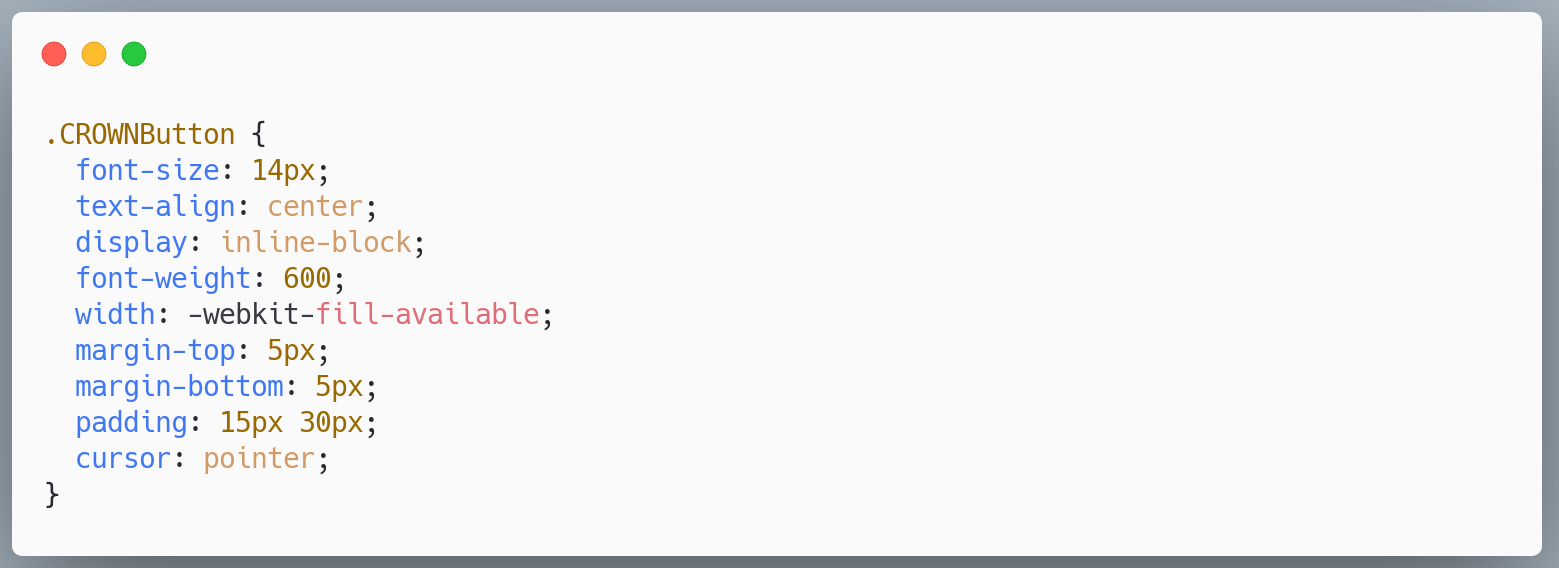
\includegraphics[width=1\textwidth]{./Imagenes/image26.png}
\newline
\newline



\subsection{ELEMENTO LABEL}
Ahora vamos a agregar el elemento Label que es un texto con el cual tenemos un formato estandarizado para tener un mejor diseño. En este elemento podemos dar parámetros de configuración como el tamaño, grosor y color que son los elementos básicos que se usan cuando estamos formateando con CSS nuestro texto. 
A continuación se presenta una lista de los parámetros y  su significado.
\newline
\begin{center}
 \begin{tabular}{ | c |  p{5cm}  | c | p{3cm} |} 
 \hline
 \textbf{Nombre} &  \textbf{Uso} &  \textbf{ Tipo de dato} &  \textbf{Valor por defecto}\\ [0.5ex] 
 \hline\hline
text 		& Este parámetro  indica el texto que vamos a mostrar.  &  Cadena de texto. 	& “I’m a label” \\  [2.5ex] 
 \hline
size 	        & Indicamos el tamaño del texto. Se cuenta con un conjunto de tamaños establecidos que se mencionan en el apartado de las constantes.       & Cadena de texto.  	& small \\[2.5ex] 
 \hline
color        & Es el color del texto.						    & Cadena de texto. 	& --black-0 \\[3.5ex] 
 \hline
 weight.   & Indicamos el grosor del texto. Se cuenta con un conjunto de tamaños establecidos que se mencionan en el apartado de las constantes.&  Cadena de texto. 	& regular \\[2.5ex] 
 \hline
\end{tabular}
\end{center}
\newline
\newline
Para el funcionamiento de la etiqueta de texto se tiene un componente de react en el cual se crea un objeto de JAVASCRIPT, se agrega la configuración del color, tamaño de texto y grosor. Finalmente se crea una etiqueta de HTML a la cual le damos nuestro objeto para que aplique el estilo y le ponemos el texto que se quiere mostrar.
\newline
\newline
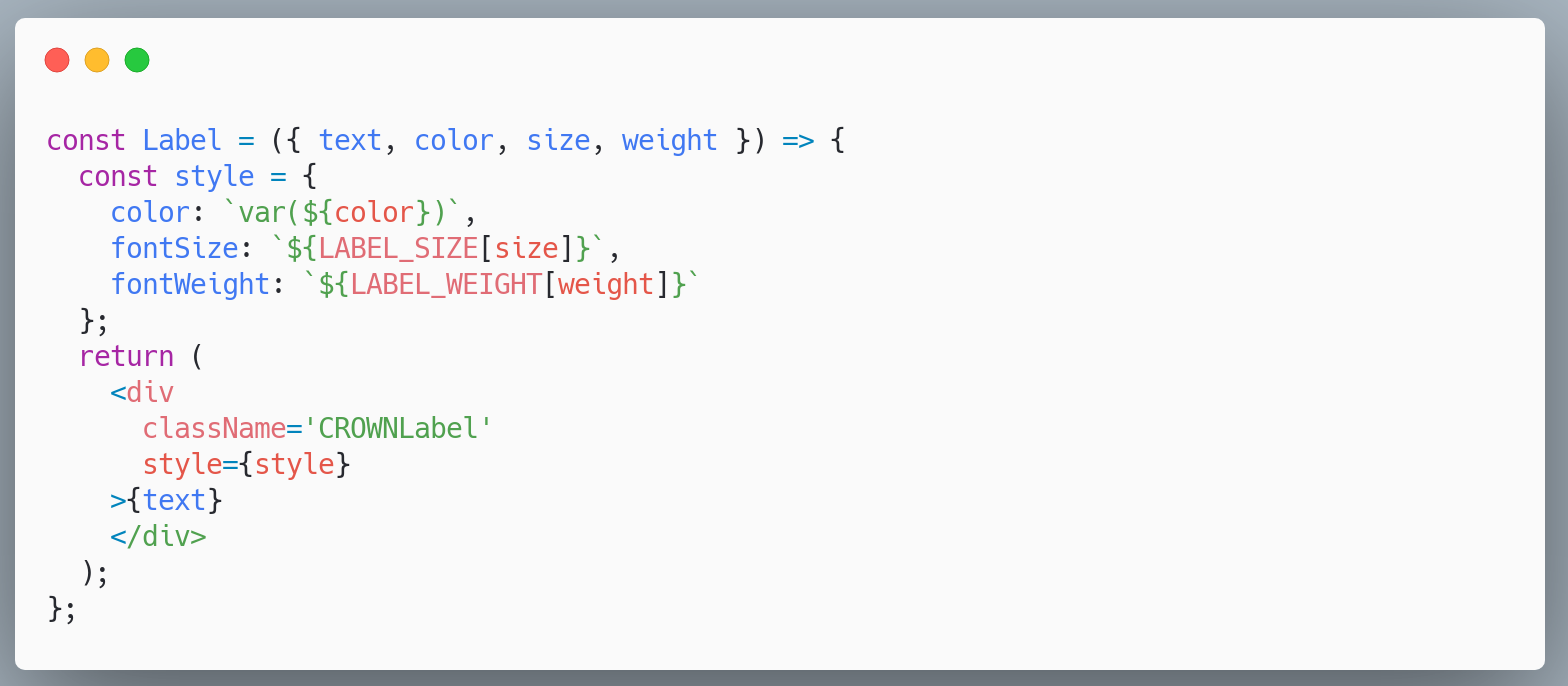
\includegraphics[width=1\textwidth]{./Imagenes/carbon-11.png}
\newline
\newline



\subsection{ELEMENTO INPUT TEX}
El input text es de utilidad para permitir la entrada de datos, y posteriormente puede ser procesado para enviarlos a algún servicio o procesarlos dentro de nuestra aplicación en donde es implementado.
Los datos de entrada que son necesarios para configurar el elemento se muestran a continuación.
\newline
\newline
\begin{center}
 \begin{tabular}{ | c |  p{5cm}  | c | p{3cm} |} 
 \hline
 \textbf{Nombre} &  \textbf{Uso} &  \textbf{ Tipo de dato} &  \textbf{Valor por defecto}\\ [0.5ex] 
 \hline\hline
placeholder &Es el texto que muestra el InputText si se desea poner.  &  Cadena de texto. 	& “Write on me!” \\  [2.5ex] 
 \hline
onChange & Es la función que va a hacer invocada cuando se escriba.     & Función vacía.  	& Función vacía.l \\[2.5ex] 
 \hline
nameState & Es el nombre con el cual se identifica en el estado.    & Cadena de texto.	& input \\[3.5ex] 
 \hline
 type   & Es la manera en como será interpretado por Input Text, estos son los que existen por defecto en HTML. Password etc.&  Cadena de texto.	& text \\[2.5ex] 
 \hline
 title  & Si se pone como “true” este agregara un Label antes del Input Text y no lo pondrá dentro.&  Booleano.	& false \\[2.5ex] 
 \hline
 extraStyle   & Si se desea agregar más estilos se puede poner el nombre de la clase CSS para poder ser manipulado.&  Cadena de texto. 	& Cadena vacía. \\[2.5ex] 
 \hline
\end{tabular}
\end{center}
\newline
\newline
La primera consideración que se tiene, es saber si se necesita tener un “Título” en nuestro Input Text, y si es así, se agrega un elemento Label antes,  para mostrar cual es el significado de nuestro label. Esto por ejemplo, si se quiere poner una entrada de texto para solicitar el correo electronico de cierta persona, esto puede estar dentro de el Input Texto denominado placeholder o afuera denominado title, por defecto title está desactivado y se activa enviando “true”.
Cuando se escribe sobre el campo de texto, este llama a la función “onChange” que recibe, se regresa el nombre de como está identificado en el estado de REACT y el valor que contiene el campo de texto.
Los demás parámetros de los estilos también son agregados en el siguiente código.
\newline
\newline
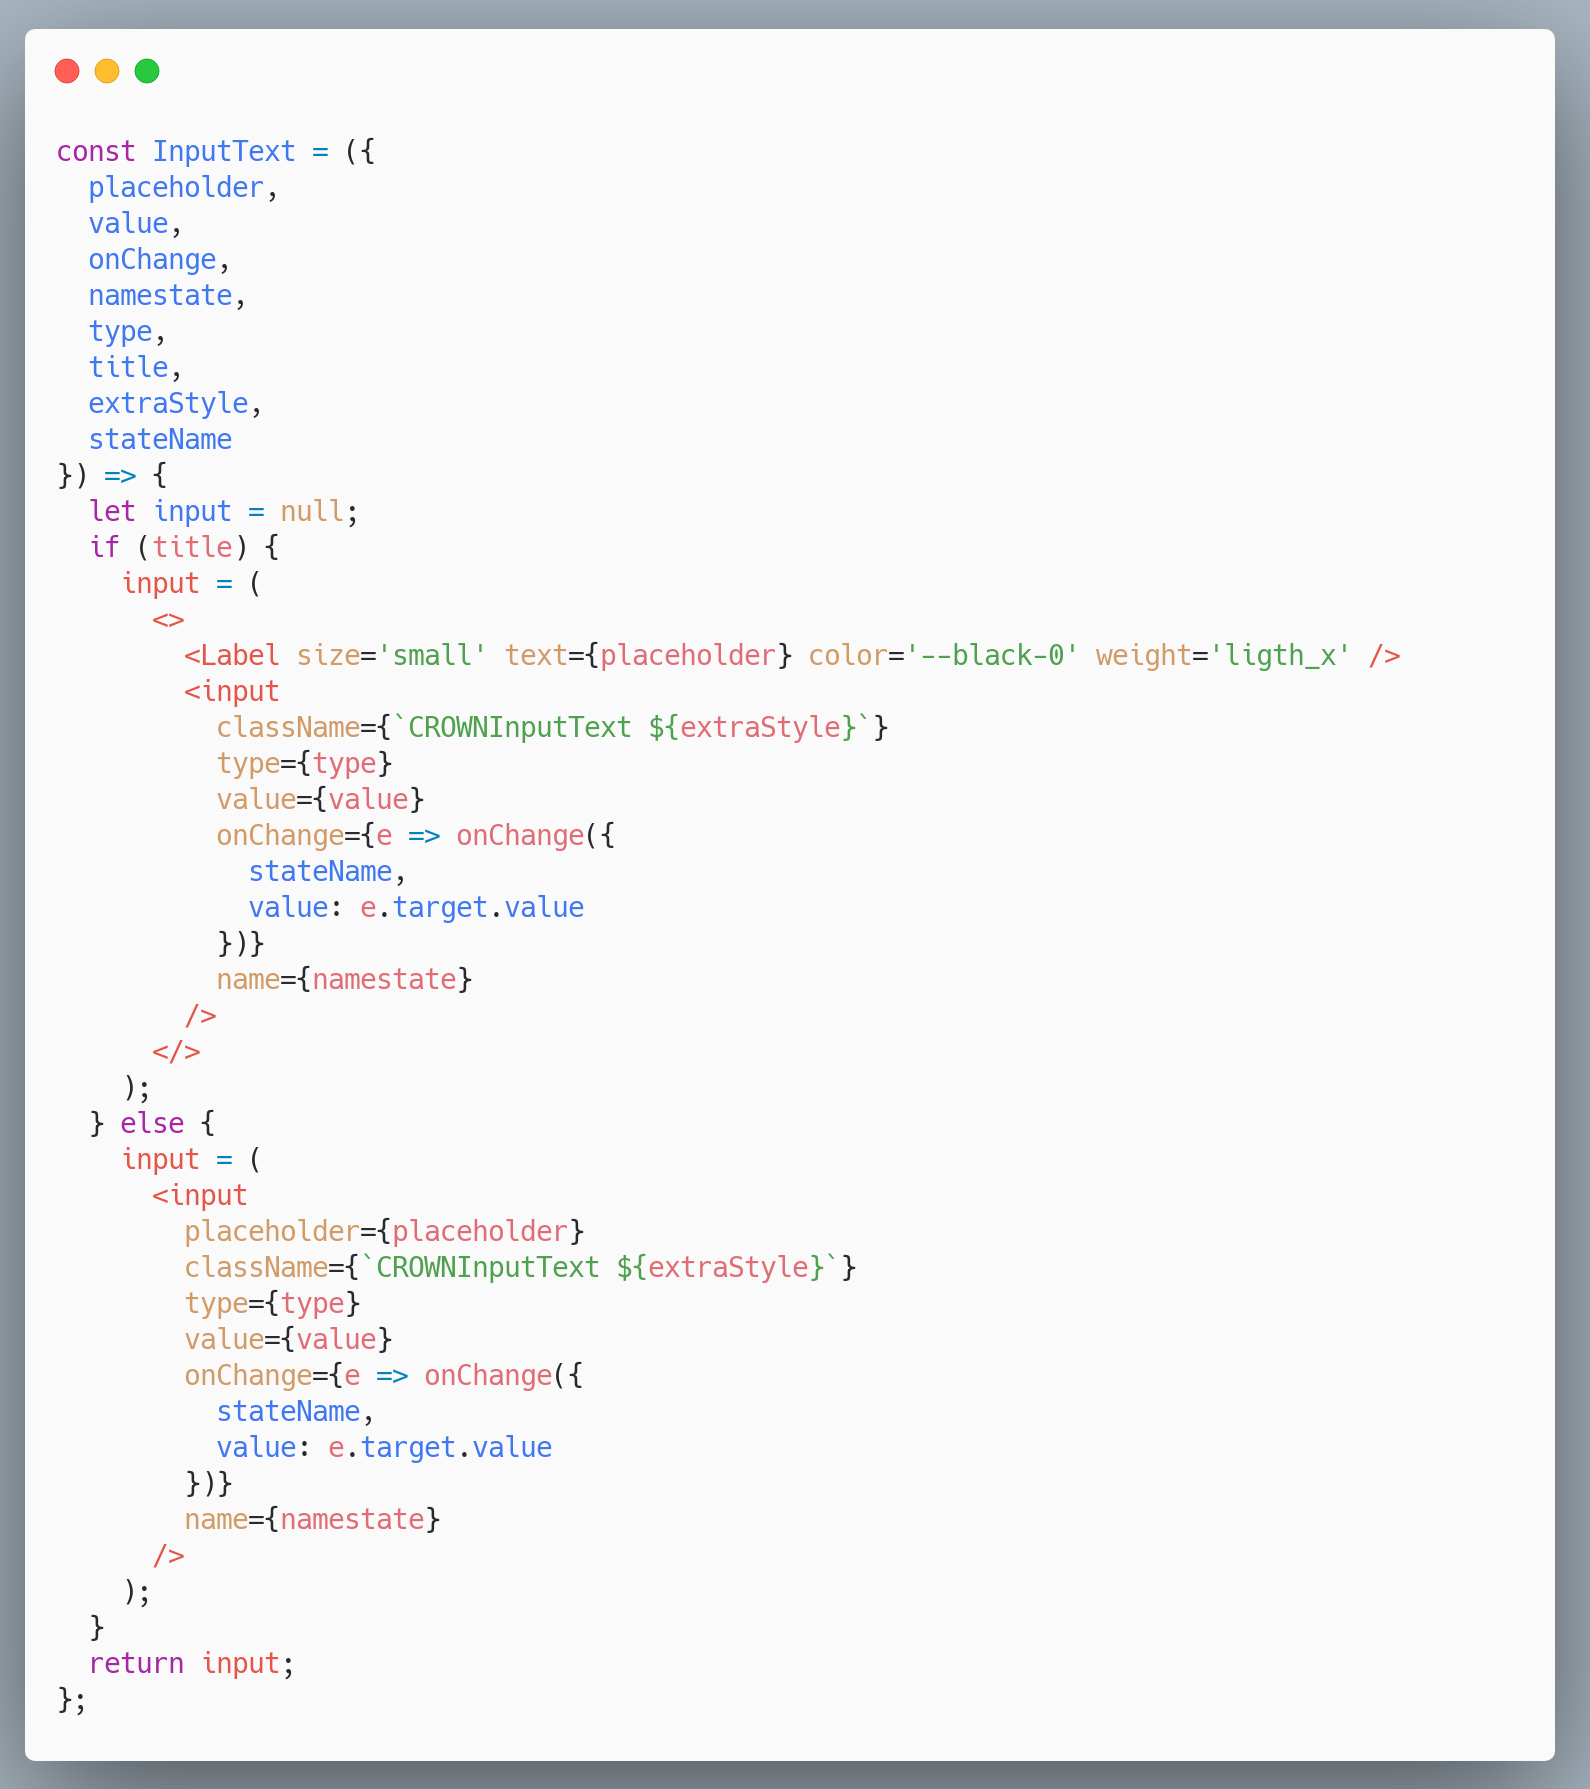
\includegraphics[width=1\textwidth]{./Imagenes/carbon-12.png}
\newline
\newline



\subsection{ELEMENTO DROP DOWN}
\subsection{ELEMENTO RADIO BUTTON}
\subsection{ELEMENTO SWITCH}
\subsection{ELEMENTO TABLE}
\subsection{ELEMENTO CHECK BOX}
\subsection{ELEMENTO IMAGE}

